% Created 2013-04-23 Tue 14:43
\documentclass[11pt,presentation]{beamer}
\usepackage[utf8]{inputenc}
\usepackage[T1]{fontenc}
\usepackage{fixltx2e}
\usepackage{graphicx}
\usepackage{longtable}
\usepackage{float}
\usepackage{wrapfig}
\usepackage{soul}
\usepackage{textcomp}
\usepackage{marvosym}
\usepackage[nointegrals]{wasysym}
\usepackage{latexsym}
\usepackage{amssymb}
\usepackage{hyperref}
\tolerance=1000
\AtBeginSection[]{\begin{frame}<beamer>\frametitle{提纲}\tableofcontents[currentsection]\end{frame}}
\providecommand{\alert}[1]{\textbf{#1}}

\title{大数据环境下信息抽取模板自动聚类与发现}
\author{计92 丘骏鹏 2009011282}
\date{指导老师:朱小燕~郝宇}
\hypersetup{
  pdfkeywords={},
  pdfsubject={},
  pdfcreator={Emacs Org-mode version 7.8.11}}

\usetheme{default}\usecolortheme{default}
\usepackage{listings}\usepackage{fontspec}\usepackage{xunicode}\usepackage{xltxtra}\usepackage{xeCJK}
\setmainfont{Times New Roman}\setmonofont{Courier New}\setCJKmainfont[BoldFont=YouYuan]{SimSun}\setCJKfamilyfont{song}{SimSun}\setCJKfamilyfont{msyh}{微软雅黑}\setCJKfamilyfont{fs}{FangSong}
\begin{document}

\maketitle



\begin{frame}<beamer>\frametitle{提纲}\tableofcontents\end{frame}
\section{选题回顾}
\label{sec-1}
\begin{frame}[fragile]
\frametitle{背景}
\label{sec-1-1}

\begin{itemize}
\item 已经获取到海量的新闻、博客、论坛等网页原始数据,需要从中提取结构化的信息
\item 做法:从已有数据中抽取模板,利用模板去抽取相似网页中的信息。
\item 目标:提取结构化信息,如新闻中的标题和正文,博客的标题和内容等,存储成以下格式,
  用于后续的处理。\tiny

\lstset{extendedchars=false,basicstyle=\ttfamily\footnotesize,escapechar=`,breaklines,language=nxml}
\begin{lstlisting}
<document>
  <news>
    <title>foobar</title>
    <content>blablabla</content>
  </news>
</document>
\end{lstlisting}
\end{itemize}
\end{frame}
\begin{frame}[fragile]
\frametitle{输入}
\label{sec-1-2}
\begin{itemize}

\item 文档集合\\
\label{sec-1-2-1}%
\lstset{extendedchars=false,basicstyle=\ttfamily\footnotesize,escapechar=`,breaklines,language=HTML}
\begin{lstlisting}
  <html>                |  <html>
    <body>              |    <body>
      <h1>Title1</h1>   |      <h1>Title2</h1>
      <p>Content1</p>   |      <p>Content2</p>
    </body>             |    </body>
  </html>               |  </html>
------------------------|--------------------------
  <html>                |  <html>
    <body>              |    <body>
      <div>             |      <div>
        <div>foo1</div> |        <div>foo2</div>
        <div>bar1</div> |        <div>bar2</div>
      </div>            |      </div>
    </body>             |    </body>
  </html>               |  </html>
\end{lstlisting}

\end{itemize} % ends low level
\end{frame}
\begin{frame}[fragile]
\frametitle{输出}
\label{sec-1-3}
\begin{columns}[t]
\begin{column}{0.5\textwidth}
\begin{itemize}

\item 抽取的模板1\\
\label{sec-1-3-1}%
\lstset{extendedchars=false,basicstyle=\ttfamily\footnotesize,escapechar=`,breaklines,language=HTML}
\begin{lstlisting}
<html>
  <body>
    <h1>?</h1>
    <p>?</p>
  </body>
</html>
\end{lstlisting}
\end{itemize} % ends low level
\end{column}
\begin{column}{0.5\textwidth}
\begin{itemize}

\item 抽取的模板2\\
\label{sec-1-3-2}%
\lstset{extendedchars=false,basicstyle=\ttfamily\footnotesize,escapechar=`,breaklines,language=HTML}
\begin{lstlisting}
<html>
  <body>
    <div>
      <div>?</div>
      <div>?</div>
    </div>
  </body>
</html>
\end{lstlisting}

\end{itemize} % ends low level
\end{column}
\end{columns}
\end{frame}
\section{系统设计与实现}
\label{sec-2}
\begin{frame}
\frametitle{框架}
\label{sec-2-1}
\begin{columns}[t]
\begin{column}{0.3\textwidth}
%% \textbf{:BMCOL:B\_ignoreheading:}
\label{sec-2-1-1}

整体框架示意图
\end{column}
\begin{column}{0.7\textwidth}
%% \textbf{:B\_ignoreheading:BMCOL:}
\label{sec-2-1-2}

    \begin{figure}[htb]
    \centering
    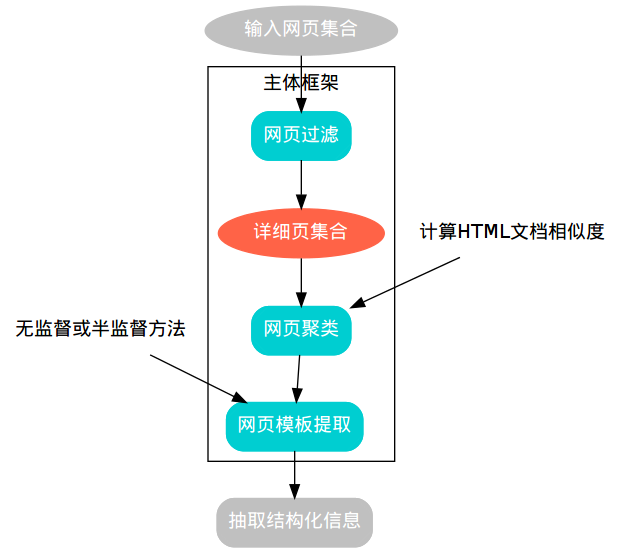
\includegraphics[width=20em,angle=0]{./framework.png}
    \caption{\label{fig:1}framework}
    \end{figure}
\end{column}
\end{columns}
\end{frame}
\begin{frame}
\frametitle{系统实现概况}
\label{sec-2-2}
\begin{itemize}

\item 主要模块实现
\label{sec-2-2-1}%
\begin{itemize}
\item $\boxtimes$ 整体框架搭建
\item $\boxtimes$ 网页过滤
\item $\boxtimes$ 网页聚类
\item $\Box$ 模板抽取
\end{itemize}

\item 进度对比
\label{sec-2-2-2}%
\begin{itemize}

\item 开题报告
\label{sec-2-2-2-1}%
\begin{itemize}
\item 5-8周:网页过滤,网页聚类和网页模板提取模块初步实现
\item 9-12周:算法修正,系统改进,结果分析
\end{itemize}

\item 实际进度
\label{sec-2-2-2-2}%
\begin{itemize}
\item 5-8周:初步的模板提取模块尚未完全实现
\item 9-12周:由于计算速度瓶颈,目前已进行了算法的优化
\end{itemize}


\end{itemize} % ends low level
\end{itemize} % ends low level
\end{frame}
\begin{frame}
\frametitle{搭建系统框架}
\label{sec-2-3}

\begin{itemize}
\item 实现语言:Java+Scala
\item 考虑到代码的重用性,采用了许多工业界广泛应用的第三方库:
\begin{enumerate}
\item \href{http://site.icu-project.org/}{icu4j} : 用于检测网页字符编码
\item \href{http://jsoup.org}{Jsoup} : HTML Parser。可以自定义Visitor来访问树的节点。
\item \href{https://github.com/twitter/util}{util-logging} : twitter包装的java.util.logging库,用于日志系统
\item \href{https://github.com/typesafehub/config}{typesafe's config} : 完成配置文件读取
\item \href{http://akka.io}{akka} : Java \& Scala的Actor模型库
\end{enumerate}
\end{itemize}
\end{frame}
\begin{frame}
\frametitle{实验数据}
\label{sec-2-4}
\begin{itemize}

\item 实验数据统计\\
\label{sec-2-4-1}%
\begin{center}
\begin{tabular}{llll}
           &  blog   &  news   &  other   \\
\hline
 文件个数  &  59998  &  81561  &  183635  \\
 总大小    &  5.4G   &  7.9G   &  18G     \\
\end{tabular}
\end{center}



    主要针对blog数据做了一些实验
\end{itemize} % ends low level
\end{frame}
\begin{frame}[fragile]
\frametitle{系统设计(1)}
\label{sec-2-5}
\begin{itemize}

\item 网页过滤模块
\label{sec-2-5-1}%
\begin{itemize}
\item 新浪博客的目录页和详细页可以用URL区分。比如某个博主的目录页为
  \tiny

\begin{verbatim}
http://blog.sina.com.cn/u/1439351555
\end{verbatim}
  \normalsize
  他的某篇文章的URL格式为
  \tiny

\begin{verbatim}
http://blog.sina.com.cn/s/blog_55cac30301016yb1.html
\end{verbatim}
  \normalsize
  因此对于博客数据可以用URL正则进行过滤
\item blog文档集合中目录页文件数为23430,详细页文件数为36568。
\end{itemize}

\end{itemize} % ends low level
\end{frame}
\begin{frame}[fragile]
\frametitle{系统设计(2)}
\label{sec-2-6}
\begin{itemize}

\item 预处理
\label{sec-2-6-1}%
\begin{itemize}
\item 去除空行、标签属性值、文本 \texttt{<\#text>} 和 \texttt{CDATA} 数据以及无用标签
  \tiny

\begin{verbatim}
<script>, <link>, <style>, <br>, <img>, <em>
\end{verbatim}
  \normalsize
\item 将树结构平坦化,降低计算复杂度。通过前序遍历 \texttt{Dom Tree} 得到tag序列:
  \tiny

\begin{verbatim}
<html>
  <body>
    <div>
      <p></p>
      <a></a>         
    </div>           
    <div></div>      
  </body>
</html>
\end{verbatim}
  \normalsize
  转化成:
  \tiny

\begin{verbatim}
<html><body><div><p></p><a></a></div><div></div></body></html>
\end{verbatim}
\end{itemize}
  

\end{itemize} % ends low level
\end{frame}
\begin{frame}
\frametitle{系统设计(3)}
\label{sec-2-7}
\begin{itemize}

\item 相似度计算\\
\label{sec-2-7-1}%
为了方便计算以及后续的模板的抽取,采用LCS作为计算相似度的基础
\begin{eqnarray*}
  c(i)(j) =
  \begin{cases}
    0 & i = 0,\: j = 0\\
    c(i-1)(j-1) + 1 & i,\: j > 0, x_i=y_j\\
    \max(c(i)(j-1), c(i-1)(j)) & i, j > 0,\: x_i \ne y_j
  \end{cases}
\end{eqnarray*}

\item Longest Common Tag Subsequence\\
\label{sec-2-7-2}%
\[
d_{LCTS}(D_1,D_2)=1-\frac{|lcts(D_1,D_2)|}{\max(|D_1|,|D_2|)}
\]

\end{itemize} % ends low level
\end{frame}
\begin{frame}[fragile]
\frametitle{重复记录的处理}
\label{sec-2-8}

\begin{itemize}
\item 网页中含有部分重复元素,这些部分是由网站后台动态生成的(Python Django):

\lstset{extendedchars=false,basicstyle=\ttfamily\footnotesize,escapechar=`,breaklines,language=Python}
\begin{lstlisting}

  <li>{{file}}</li>

\end{lstlisting}
\item 简单的方法:去掉这些标签,在比较过程中不予考虑。但这种方法无法处理更复杂的
     情况。如一个 \texttt{<div>} 标签下的子树(Data Record)。
\item 后缀树(SuffixTree)
\begin{itemize}
\item Trie的一个变种,可以快速找到字符串中的重复子串
\item 快速算法可以在\(O(n)\) 时间内构建: \\\footnotesize\em
       Ukkonen, Esko. ``On-line construction of suffix trees.'' Algorithmica 14.3
       (1995): 249-260.
\end{itemize}
\item 由于采用前序遍历,可以保证子树在序列上是连续的
\end{itemize}
\end{frame}
\begin{frame}[fragile]
\frametitle{后缀树}
\label{sec-2-9}

\begin{itemize}
\item 对于字符串mississippi:
     \tiny

\begin{verbatim}
T1  = mississippi        tree-->|---mississippi                T1
T2  = ississippi                |                             
T3  = ssissippi                 |---i-->|---ssi-->|---ssippi   T2
T4  = sissippi                  |       |         |           
T5  = issippi                   |       |         |---ppi      T5
T6  = ssippi                    |       |                     
T7  = sippi         =>          |       |---ppi                T8
T8  = ippi                      |                             
T9  = ppi                       |---s-->|---si-->|---ssippi    T3
T10 = pi                        |       |        |            
T11 = i                         |       |        |---ppi       T6
                                |       |                     
                                |       |---i-->|---ssippi     T4
                                |               |             
                                |               |---ppi        T7
                                |                             
                                |---p-->|---pi                 T9
                                        |                     
                                        |---i                  T10
\end{verbatim}
     \normalsize
\item 任一到内部节点的路径都是字符串中重复的子串
\end{itemize}
\end{frame}
\begin{frame}
\frametitle{聚类算法}
\label{sec-2-10}
\begin{itemize}

\item 实现了一个简单的层次聚类算法
\label{sec-2-10-1}%

\item 过程
\label{sec-2-10-2}%
\begin{itemize}
\item 每个文档开始时单独为一类,并作为该类的中心点
\item 选择中心点距离最近的两个类进行合并
\item 更新类中心点:选择距离其他点距离之和最小的点作为类的新中心点,重复以上过程
\end{itemize}

\item 算法特点
\label{sec-2-10-3}%
\begin{itemize}
\item 只需要计算一次文档集合相互之间的相似度
\item 阈值较难设置
\end{itemize}
\end{itemize} % ends low level
\end{frame}
\section{系统优化}
\label{sec-3}
\begin{frame}
\frametitle{动机}
\label{sec-3-1}

\begin{enumerate}
\item LCS的动态规划算法的时间复杂度为\(O(mn)\) ,空间复杂度也是\(O(mn)\)
\item 文档数很大,运行时需载入内存,需要尽量减少空间复杂度
\item 假设每运行一次算法的时间为t,以最小的文档集合blog为输入(数目约为60000篇),则
   计算文档集合中两两之间距离的总时间约为:
   \[
   \frac{60000^2}{2 * 3600}*t=5*10^5*t
   \]
   取\(t=0.001s\),则总时间为\(5*10^5*0.001=500h\)。
\end{enumerate}
\end{frame}
\begin{frame}
\frametitle{优化空间}
\label{sec-3-2}

\begin{itemize}
\item 动态规划原理式
     \begin{eqnarray*}
       c(i)(j) =
       \begin{cases}
         0 & i = 0,\: j = 0\\
         c(i-1)(j-1) + 1 & i,\: j > 0, x_i=y_j\\
         \max(c(i)(j-1), c(i-1)(j)) & i, j > 0,\: x_i \ne y_j
       \end{cases}
     \end{eqnarray*}
     以行优先遍历为例:实际上我们在计算每一个点的值时,依赖的信息只包括这一行之
     前已计算出的点和前一行的点,所以只需要两个一维数组即可。空间复杂度降低为
     \(O(n)\)。
\end{itemize}
\end{frame}
\begin{frame}[fragile]
\frametitle{优化时间}
\label{sec-3-3}

\begin{itemize}
\item 减小运行时间的有效办法是压缩tag序列长度。
\begin{enumerate}
\item 预处理已经去掉了很多无用标签
\item \texttt{<tagName></tagname>} 可以用 \texttt{(tagName, depth)} 来表示,相当于将HTML转换为
        S-expression。\footnotesize

\begin{verbatim}
<html>                          <=>  (html
 <body>                         <=>    (body
  <div>                         <=>      (div
   <p></p></div></body></html>  <=>        (p))))
\end{verbatim}
        \normalsize
\end{enumerate}
\item 用途:由于大部分的标签都是成对的,因此这样大概可以减少一半的tag序列长度。
\item 标签比较时加入深度信息:
     \footnotesize

\begin{verbatim}
node1.tagName = node2.tagName && node1.depth = node2.depth
\end{verbatim}
     \normalsize
\end{itemize}
\end{frame}
\begin{frame}
\frametitle{优化计算方式(1)}
\label{sec-3-4}

\begin{itemize}
\item 在以上优化的基础上,两两之间进行一次计算需要的时间为\(0.001\sim 0.002s\)。
\item 之前已经计算过,在\(t=0.001s\)的情况下,计算一次blog集合中所有文档相互之间
     的距离需要500小时。
\item 优化计算方式:采用多线程进行计算。
\end{itemize}
\end{frame}
\begin{frame}
\frametitle{优化计算方式(2)}
\label{sec-3-5}
\begin{itemize}

\item 采用Actor库进行实现
\label{sec-3-5-1}%
\begin{itemize}
\item 一种并行计算的模型,每个Actor是完全独立的,相互间采用异步、非阻塞的消息传递
      进行通信
\item 优点:可以避免使用全局状态、锁、信号量等一些低级的同步原语;有封装好的线程
      调度算法,不需要手动对线程进行管理,简化任务的分割。
\end{itemize}

\item 具体实现
\label{sec-3-5-2}%
\begin{itemize}

\item 将该区域用等距的横线和纵线分割,然后将这些区域通过调度器分发给每个可用的Actor进行计算。调度算法采用简单的Round-Robin。
\label{sec-3-5-2-1}%
\end{itemize} % ends low level
%% \textbf{:B\_ignoreheading:BMCOL:}
\label{sec-3-5-2-2}

\begin{figure}[htb]
\centering
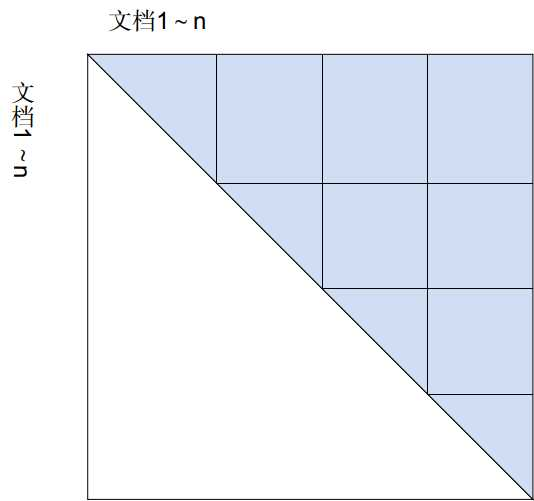
\includegraphics[width=0.3\textwidth,angle=0]{./图片1.jpg}
\caption{\label{fig:1}示意图}
\end{figure}
\end{itemize} % ends low level
\end{frame}
\begin{frame}
\frametitle{优化距离计算}
\label{sec-3-6}

\begin{itemize}
\item 考虑深度的影响,离根节点越近的标签权重越大
\item 修改LCS算法,\(f(x)\)是一个与当前节点深度\(x\)有关的函数:
     \begin{eqnarray*}
       c(i)(j) =
       \begin{cases}
         0 & i = 0,\: j = 0\\
         c(i-1)(j-1) + f(x_i.depth) & i,\: j > 0, x_i=y_j\\
         \max(c(i)(j-1), c(i-1)(j)) & i, j > 0,\: x_i \ne y_j
       \end{cases}
     \end{eqnarray*}
\item 同时修改距离计算公式
     \[
     d_{LCTS}(D_1,D_2)=1-\frac{|lcts(D_1,D_2)|}{\max(\sum\limits_{n\in
     D_1}{f(n.depth)},\sum\limits_{n\in D_2}{f(n.depth)})}
     \]
\end{itemize}
         
\end{frame}
\section{初步结果}
\label{sec-4}
\begin{frame}
\frametitle{实验设置}
\label{sec-4-1}
\begin{itemize}

\item 在实验室的服务器上进行实验,机器配置为16个逻辑CPU+24G内存
\label{sec-4-1-1}%

\item 由于以上限制,目前在小数据量上做实验:从blog中抽取出了1000个文档作为实验的文档集合
\label{sec-4-1-2}%
\end{itemize} % ends low level
\end{frame}
\begin{frame}
\frametitle{实验结果}
\label{sec-4-2}

\begin{itemize}
\item 直接聚类:在阈值为0.3的情况下,所有文档聚成一类,通过手工可以大致确定正确性
\item 验证可行性:加入噪音
\begin{itemize}
\item 在详细页文档中加入目录页、404错误页等噪音
\item 聚类结果:在阈值为0.3的情况下,文档被聚成3类,分别是详细页,目录页和404错
      误页
\end{itemize}
\item 初步分析:
\begin{itemize}
\item 阈值设置:目前暂无法确定合适阈值将两个文档分为不同的两类
\item 评价:需要根据最后的模板抽取结果来判断
\end{itemize}
\end{itemize}
\end{frame}
\section{后期工作}
\label{sec-5}
\begin{frame}
\frametitle{后期工作目标}
\label{sec-5-1}
\begin{itemize}

\item 实现模板抽取
\label{sec-5-1-1}%
\begin{itemize}
\item 利用计算出的公共字串及tag的深度信息反向构建出树结构,作为该类的模板
\item 采取少量标注进行半监督学习
\end{itemize}

\item 新文档分类
\label{sec-5-1-2}%
\begin{itemize}
\item 归为已有的一类,利用该类的模板抽取文档内容
\item 归为新的类,计算新的模板
\end{itemize}

\item 结果评价
\label{sec-5-1-3}%
\begin{itemize}
\item 根据模板抽取结果,调整实验参数
\end{itemize}
\end{itemize} % ends low level
\end{frame}

\end{document}